The electroweak process \Wgstar\ is normally covered in Monte Carlo
simulations as a part of the \WZ\ process. Questions were raised if
the low mass region is adequately covered since the \WZ\ Madgraph
simulations have a generator level cut $m_{\gamma^*}>12$ and there is
significant rate of events at lower values~\cite{wgstar}.  \WZ\
and \Wgstar\ processes contribute as background to the Higgs signal in
the case one of the three leptons in the final state is not
detected. We have simulated the low mass part of \Wgstar\ using a
leading order matrix element Monte Carlo (Madgraph). The generator
level selection requirements were relaxed: require two leptons each
with $\pt>5$~\GeV{} with no restrictions on the third one, consider
electrons and muons to be massive to properly simulate the kinematic
cutoff. The key question is to observe the process in data and
validate the simulation. In particular we need to measure the
cross-section of the process to have reliable predictions for the
background outside the control region.

We can consider separately the two cases where the lepton pair from
the \Astar are electrons or muons. For the generator level selections
mentioned above the cross section for
the \ensuremath{l^{\pm}e^{+}e^{-}} final state
(with \ensuremath{l^{\pm}}=\ensuremath{\mu^{\pm}}
or \ensuremath{e^{\pm}} being the lepton from the \W\ decay) is larger
by a factor $\sim3$ with respect to
the \ensuremath{l^{\pm}\mu^{+}\mu^{-}} case due to the lower
production threshold (defined by \ensuremath{2M_{l}}) and the steep
rising of \ensuremath{d\sigma/dM_{\gamma}}.  The leptons originated
from the virtual photon feature small opening angle and small
invariant mass.  At least one of the two leptons is soft with an
average \pt\ of $\sim5$ GeV.  In the \ensuremath{l^{\pm}e^{+}e^{-}}
case the way of faking the signal is similar to the \wgamma\
background when the photon converts in the material close to the
interaction vertex (it can be seen as a sort of ``prompt''
conversion).  For the \ensuremath{l^{\pm}\mu^{+}\mu^{-}} final state,
the low \pt\ of the softest muon often prevents it from reaching the
muon stations and thus to be identified as a muon.

To measure the production rate of \Wgstar\ in data we focused only on
the \ensuremath{l^{\pm}\mu^{+}\mu^{-}} final state, since the large
background from QCD makes it hard to extract signal in
the \ensuremath{l^{\pm}e^{+}e^{-}} case.  The \Wgstar\ control region
selection has been optimized for high purity.  The following
selections have been applied:
\begin{itemize}
\item 
the muon pair associated to the virtual photon needs to have opposite
charge. In the case of \ensuremath{\mu\mu\mu} final state, the pair
with lowest mass is assumed to originate from the \Astar.
\item 
the muon isolation is redefined to exclude muons from the isolation
energy calculation to reconstruct events with two muons closer
than \delR=0.3.
\item 
to suppress top background events with less than 2 jets are
considered and anti b-tagging is required for all jets
with \ensuremath{p_\mathrm{T}>10} GeV.
\item 
to suppress QCD background minMet$>20$ and \mt$>20$ (where \mt is
computed from the \W's lepton and the \met).
\item 
\ensuremath{M_{\mu\mu}<12} GeV.
\end{itemize} 

The upper bound on the di-muon mass is set to get rid of the
interference between \Wgstar\ and \ensuremath{\W\Zstar}.  The Monte
Carlo used for the \WZ\ process includes both \Astar\ and \Zstar\
contributions and takes properly into account the interference between
them.  The plot in Figure \ref{fig:WgammaStarMass} compares the mass
distributions of the muon pair associated with the virtual photon for
data and Monte Carlo once all the selections listed above are applied
but \ensuremath{M_{\mu\mu}<12} GeV.  The data correspond to an
integrated luminosity equal to 2.97\ifb.

\begin{figure}[hbt]
\begin{center}
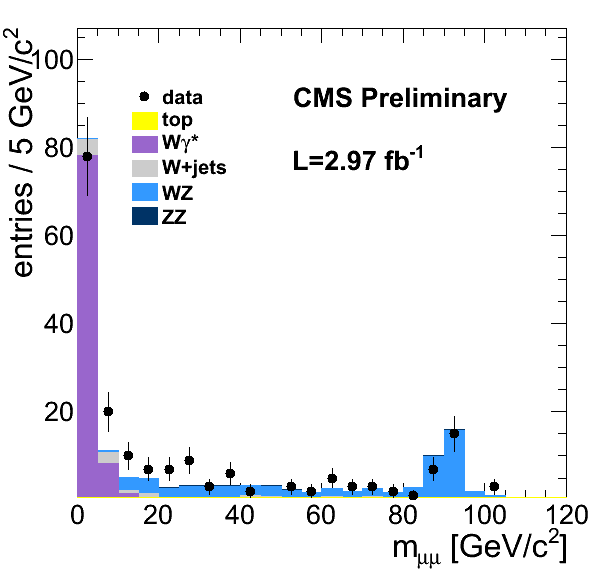
\includegraphics[width=0.5\linewidth]{figures/gammaMass_m120.png} 
\caption{\label{fig:WgammaStarMass}\protect Comparison of data and Monte Carlo for  
mass distributions of the muon pair associated with the virtual
photon.  All the selections defining the \Wgstar\ control region are
applied but \ensuremath{M_{\mu\mu}<12} GeV.}
\end{center}
\end{figure}

The plots in Figure \ref{fig:WgammaStar}, displaying data and MC
distributions for the muon pair associated with the virtual photon,
(left: opening angle, center: di-muon mass, right: \pt\ of the softest
muon) assess the compatibility of the data belonging to the control
region with the expectations from the \Wgstar\ Monte Carlo.  
The contribution from other backgrounds is very limited, 
the only process which is not completely negligible is $\Wjets$
which is computed directly from data by means of the fake rate
method described in section \ref{sec:bkg_fakes}.
A small difference is observed between the data and MC shapes
for the mass of the virtual photon candidate; 
as this mismodelling was also observed in 2011 data we will discuss the
related systematics in the following.

\begin{figure}[hbt]
\begin{center}
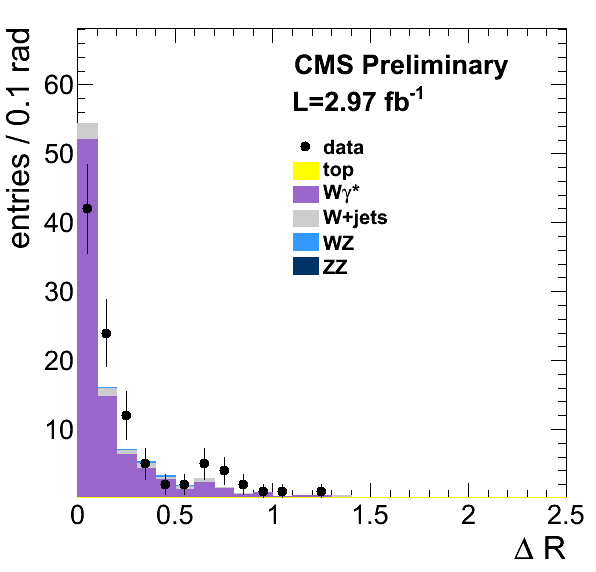
\includegraphics[width=0.3\linewidth]{figures/gammaDR_m12.png} 
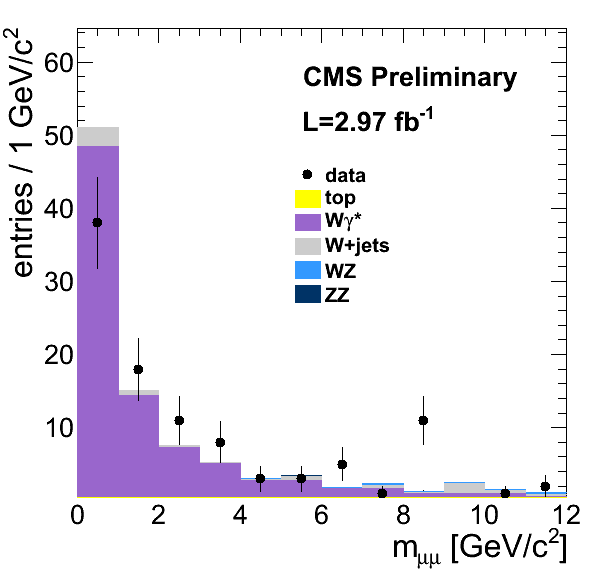
\includegraphics[width=0.3\linewidth]{figures/gammaMass_m12.png}
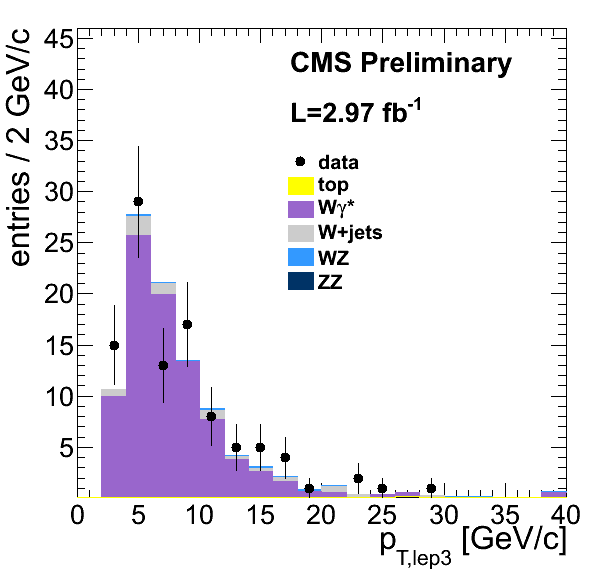
\includegraphics[width=0.3\linewidth]{figures/gammaLep3Pt_m12.png}
\caption{\label{fig:WgammaStar}\protect Comparison of data and Monte Carlo for three 
main distributions of the muons associated with the virtual photon in
the \Wgstar~ control region.  Left: opening angle (\delR).  Center:
di-muon mass.  Right:. softest muon \pt.}
\end{center}
\end{figure}

\begin{table}[!hbt]
\begin{center}
\begin{tabular}{|c|c|c|c|c|c|c|}
\hline
& \multicolumn{2}{|c|}{\ensuremath{e\mu\mu}} & \multicolumn{2}{|c|}{\ensuremath{\mu\mu\mu}} & \multicolumn{2}{|c|}{\ensuremath{l\mu\mu}} \\
\hline
& SS & OS & SS & OS & SS & OS \\
\hline
data yields & 12 & 17 & 35 & 37 &  49 &  52\\
\hline
background & 1.8 & 1.0 & 2.3 &  3.4 &  5.2 & 3.3\\
\hline
(raw) \Wgstar~ MC yields & $7.7 \pm 0.5$ & $7.7 \pm 0.4$ & $20.1 \pm 0.7$ & $22.9 \pm 0.8$ & $30.6 \pm 0.9$ & $27.8 \pm 0.8$ \\
\hline
\hline
{\em k-}factor & \multicolumn{2}{|c|}{1.69} & \multicolumn{2}{|c|}{1.54} & \multicolumn{2}{|c|}{1.58} \\
\hline
\end{tabular}
\caption{Results of the measurements in the \Wgstar control region.
{\em k-}factors are computed as ratios between the data yields and the
MC predictions.  Results are shown separately for \ensuremath{e\mu\mu}
and \ensuremath{\mu\mu\mu} final states in the first two columns,
whereas the third one consider them together.  
For each final state yields are shown separately for same sign and opposite sign
of the two highest \pt leptons. 
The data yields correspond to \ensuremath{L=2.97\ifb}.
\label{tab:wgamma}}
\end{center}
\end{table}

Table \ref{tab:wgamma} summarizes the results of the \Wgstar~
measurement and the normalization of the corresponding Monte
Carlo. The measured {\em k}-factor is 1.6 and it is fully consistent with
the one measured with the 2011 dataset ~\cite{HWW2011}.
The {\em k}-factors measured for other EWK processes computed at the leading
order resulted very similar to the one obtained here, giving therefore 
further confidence on the accuracy of the Monte Carlo simulation.  
As a further cross check, the event yields for same sign and opposite sign 
(where the pair of highest \pt leptons is considered) have been looked at in data:
as shown in table \ref{tab:wgamma}, a very good agreement is observed for each final 
state.

To estimate the systematic uncertainty related to the data versus Monte Carlo 
disagreement on the virtual photon mass shape (most likely due to mismodeling
of reconstruction efficiency of close-by muon one of which at very low \pt),
the scale factor has been computed in sub-regions of the mass spectrum and compared to what
obtained from the full range. 
We performed the same analysis on 2011 data obtaining almost identical results as
from the 2012 dataset (four scale factors estimations): 
the scale factor in the [0-2] GeV mass range results smaller ($\sim1.3$),
whereas in the range [2-12] it results larger ($\sim2.2$).
To account for this effect we assign a systematic uncertainty corresponding to
the average of the spreads of the fours estimates w.r.t the central value, obtaining
an error of $30\%$. 


